\documentclass[pdftex,a4paper]{article}
\usepackage{a4wide}
\usepackage[english]{babel}
\usepackage[utf8]{inputenc}
\usepackage[T1]{fontenc}
\usepackage{graphicx}
\usepackage{multirow}
\usepackage{multicol}
\usepackage{wrapfig}
\usepackage{pslatex}

\sloppy

\begin{document}
\title{Analysis of the ROOT Persistence I/O Memory Footprint in LHCb}
\author{
  Ivan Valen\v{c}\'{i}k\\
  \makeatletter
  \texttt{ivan.valencik@cern.ch}\\
  \\
  \small{Supervisor}\\
  Markus Frank\\
  \texttt{markus.frank@cern.ch}\\
  \\
  
\includegraphics[width=0.1\textwidth]{Ivan_Valencik_RootCnv_opt_lhcb.jpg}
  \makeatother
}
\date{\today}

\maketitle

\begin{abstract}
A ROOT conversion service that provides persistence in the GAUDI framework has a number of optimization parameters. LHCb produces smaller events with higher frequency than other LHC experiments, thus optimization done for them is not always relevant. In order to measure performance of various settings we introduce a new service and tools to analyze them. We explore the parameter space and based on the gathered data we come to an optimization decision.
\end{abstract}

\section{Introduction}
The GAUDI data processing framework \cite{frank2000} used by the LHCb experiment uses ROOT I/O to persist data resulting from particle collisions in the LHC collider. The ROOT I/O mechanism for event data offers various parameters, which have to be optimized depending on the structure of the data. This optimization has substantial influence on both event data writing and reading for further analysis. Varying these parameters affects memory usage, required processor time and the data file size. In this paper we present a performed analysis of the parameter space with LHCb event data and tools developed to obtain the measurements.

The paper is structured as follows. Section \ref{sec:cnvsvc} contains an overview of ROOT Conversion Service. In section \ref{sec:perfmon} we present a developed system resource usage monitoring service. In section \ref{sec:perftest} is described a methodology of the measuring. In section \ref{sec:measurements} are obtained results and in section \ref{sec:findings} we analyze them and come to an optimization decision. In section \ref{sec:conclusion} is given conclusion.

\section{ROOT Conversion Service}
\label{sec:cnvsvc}
Data persistence in GAUDI framework is provided by conversion services. The ROOT conversion service allows persistence of event data to ROOT files. This service allows to modify multiple parameters and hence to optimize the performance of the ROOT I/O mechanism. A basket size represents an initial amount of memory given to the ROOT. This memory is reevaluated during the run after 10th processed event. The default value is 40 MB. A splitting level indicates whether data of one event should be written to the disk together or rather divided to more primitive parts. The default value is 99, e.g. do as much splitting as possible. The tree branch buffer size sets the amount of memory used by one single branch in a ROOT tree. The default value is 32 kB. These parameters can be set only when the tree is being written to the disk and they are used implicitly by ROOT also when the data are read back.

\section{ROOT Performance Monitor}
\label{sec:perfmon}
When optimizing we are interested in the following features: memory usage, processor time, resulting file size and the behavior in the presence of multiple streams. In order to measure these quantities we developed a performance monitoring service that collects these data and persists them in a ROOT file. The measurements are done always in the beginning of the event processing and one measurement is done in the in stop and finalize methods of the service to get an idea about FSR.

The following observables are measured in every record:
\begin{multicols}{2}
\begin{itemize}
  \item virtual memory size (vsize)
  \item resident set size (rss)
  \item processor time scheduled in user mode
  \item processor time scheduled in kernel mode
  \item elapsed time
  \item file sizes
\end{itemize}
\end{multicols}

The service can be added to any service using RootCnv for data persistence just by adding the python module to the execution line, e.g. \verb|python `which gaudirun.py` stripping.py RootPerfMon.py|.

\section{Performance Test}
\label{sec:perftest}
In order to explore the whole parameter space we performed a sweep over the parameter space. To do this we created a python module PerfTest that executes a number of copy and read jobs with various parameters. A series of computations should be always run on one computer at once or in one batch job, because various computers can differ significantly in their computational power. It has been observed that it is not uncommon for some computers to require twice the time to finish the job.

In the test setup we were copying 10 000 events per stream and then reading back all copied events. In comparison, a stripping job has 14 streams which are typically copying only fraction or a few percents of the reconstructed data. When running the copy job with various fractions of the copied data we could see that it is not necessary to copy all data to reach maximum memory usage, as it depends only marginally on the fraction of the copied data.

The python module PerfTest should be executed with a help of provided bash script \verb|perftest.sh|. The usage of the module is described in its help which can be accessed by the command \verb|./perftest.sh help|. In the module it is possible to choose the number of events, the number of output streams in one job, the used basket size, the tree branch buffer size and the split level. The test can be run also only for reading or copying.

\section{Measurements}
\label{sec:measurements}
We performed a number of sweeps. In table \ref{tab:1copystream} is depicted the memory usage before and after writing File Summary Records (FSR), runtime and output file size. These values were observed in one specific job; however the differences and trends were consistent in all executions of the sweeps. The values cannot be averaged because of the different computers and their loads during the tests. In table \ref{tab:2copystreams} shows the same measurements for 2 simultaneous streams. We executed these sweeps also for 5 and 10 streams to confirm that the effects of adding 1 stream are the same. The obtained data confirmed this premise.

The table \ref{tab:smallvalues} provides a closer look of the behavior when using small a small value for the basket size and the tree buffer size. Table~\ref{tab:1readstream} shows the memory usage and the time consumption of read jobs performed in the sweep. While the memory usage is very consistent among the various measurements, the duration of job varies a lot and it is not possible deduce a conclusion from the values shown in the table.

\begin{table}
\centering
\caption{\small{Memory usage and runtime of 1 copying stream.}}
\label{tab:1copystream}
\begin{tabular}{|c|c|c|c|c|c|}
  \hline
  \multirow{2}{*}{1 stream} & split level & \multicolumn{2}{|c|}{0} & \multicolumn{2}{|c|}{99} \\
  \cline{2-6}
  & buffer size & 2 kB & 32 kB & 2 kB & 32 kB \\
  \hline
  \multirow{4}{2 cm}{basket size\\2 MB} & vsize (MB) & 660 & 660 & 662 & 681 \\
  & +FSR (MB) & 660 & 688 & 665 & 708 \\
  & time (s) & 373 & 395 & 790 & 773 \\
  & file size (MB) & 84.0 & 83.7 & 96.9 & 96.8 \\
  \hline
  \multirow{4}{2 cm}{basket size\\20 MB} & vsize (MB) & 687 & 685 & 687 & 702 \\
  & +FSR (MB) & 687 & 712 & 687 & 726 \\
  & time (s) & 322 & 486 & 384 & 405 \\
  & file size (MB) & 80.4 & 80.4 & 84.9 & 84.9 \\
  \hline
  \multirow{4}{2 cm}{basket size\\40 MB} & vsize (MB) & 709 & 714 & 709 & 727 \\
  & +FSR (MB) & 709 & 735 & 709 & 747 \\
  & time (s) & 342 & 343 & 401 & 400 \\
  & file size (MB) & 80.2 & 80.2 & 84.4 & 84.5 \\
  \hline
\end{tabular}
\end{table}

\begin{table}
\centering
\caption{\small{Memory usage and runtime of 2 copying streams.}}
\label{tab:2copystreams}
\begin{tabular}{|c|c|c|c|c|c|}
  \hline
  \multirow{2}{*}{2 streams} & split level & \multicolumn{2}{|c|}{0} & \multicolumn{2}{|c|}{99} \\
  \cline{2-6}
  & buffer size & 2 kB & 32 kB & 2 kB & 32 kB \\
  \hline
  \multirow{4}{2 cm}{basket size\\2 MB} & vsize (MB) & 678 & 678 & 682 & 703 \\
  & +FSR (MB) & 679 & 747 & 705 & 772 \\
  & time (s) & 546 & 608 & 1542 & 1480 \\
  & file size (MB) & 84.0 & 96.9 & 83.7 & 96.8 \\
  \hline
  \multirow{4}{2 cm}{basket size\\20 MB} & vsize (MB) & 731 & 727 & 735 & 746 \\
  & +FSR (MB) & 731 & 796 & 746 & 811 \\
  & time (s) & 458 & 430 & 569 & 570 \\
  & file size (MB) & 80.4 & 84.9 & 80.4 & 84.9 \\
  \hline
  \multirow{4}{2 cm}{basket size\\40 MB} & vsize (MB) & 776 & 778 & 772 & 788 \\
  & +FSR (MB) & 776 & 842 & 791 & 850 \\
  & time (s) & 488 & 458 & 544 & 639 \\
  & file size (MB) & 80.2 & 84.4 & 80.2 & 84.5 \\
  \hline
\end{tabular}
\end{table}

\begin{table}
\centering
\caption{\small{Memory usage and runtime of 1 copy stream with small settings.}}
\label{tab:smallvalues}
\begin{tabular}{|c|c|c|c|c|c|c|c|}
  \hline
  \multirow{2}{*}{1 stream} & split level & \multicolumn{3}{|c|}{0} & \multicolumn{3}{|c|}{99} \\
  \cline{2-8}
  & buffer size & 1 kB & 2 kB & 4 kB & 1 kB & 2 kB & 4 kB \\
  \hline
  \multirow{3}{2 cm}{basket size\\1 MB} & vsize (MB) & 657 & 657 & 657 & 660 & 661 & 661 \\
  & +FSR (MB) & 657 & 657 & 657 & 660 & 665 & 684 \\
  & time (s) & 634 & 576 & 593 & 1705 & 1679 & 1539 \\
  \hline
  \multirow{3}{2 cm}{basket size\\2 MB} & vsize (MB) & 659 & 660 & 659 & 662 & 662 & 663 \\
  & +FSR (MB) & 659 & 660 & 659 & 662 & 664 & 683 \\
  & time (s) & 550 & 691 & 836 & 1032 & 1158 & 1181 \\
  \hline
  \multirow{3}{2 cm}{basket size\\4 MB} & vsize (MB) & 663 & 663 & 664 & 664 & 665 & 666 \\
  & +FSR (MB) & 663 & 663 & 664 & 664 & 667 & 686 \\
  & time (s) & 653 & 746 & 763 & 987 & 1008 & 944 \\
  \hline
\end{tabular}
\end{table}

\begin{table}
\centering
\caption{\small{Memory Usage and Runtime of 1 Copying Stream}}
\label{tab:1readstream}
\begin{tabular}{|c|c|c|c|c|c|}
  \hline
  \multirow{2}{*}{1 stream} & split level & \multicolumn{2}{|c|}{0} & \multicolumn{2}{|c|}{99} \\
  \cline{2-6}
  & buffer size & 2 kB & 32 kB & 2 kB & 32 kB \\
  \hline
  \multirow{2}{2 cm}{basket size\\2 MB} & vsize (MB) & 463 & 463 & 465 & 467 \\
  & time (s) & 23 & 27 & 28 & 30 \\
  \hline
  \multirow{2}{2 cm}{basket size\\20 MB} & vsize (MB) & 489 & 491 & 490 & 485 \\
  & time (s) & 25 & 36 & 27 & 24 \\
  \hline
  \multirow{2}{2 cm}{basket size\\40 MB} & vsize (MB) & 507 & 510 & 513 & 507 \\
  & time (s) & 20 & 23 & 26 & 28 \\
  \hline
\end{tabular}
\end{table}

\section{Results}
\label{sec:findings}
Looking at the table \ref{tab:1copystream} and \ref{tab:2copystreams} we can see that 1 stream costs more than 60 MB when current settings are used, i.e. 40 MB basket size, 32 kB tree branch buffer and splitting is on. Another 40 MB are necessary to write FSR with these settings. This configuration is marked with a blue triangle in figure \ref{fig:vsizeXcpu}. This figure depicts memory and processor time required by various configurations of parameters tested in the sweep.

The cost of 1 stream is only about 19 MB when we use low basket size, low tree branch buffer and no splitting. This configuration is depicted in figure  \ref{fig:vsizeXcpu} in the green circle. Another advantage of this configuration is that the increase of memory for writing FSR is negligible.

This difference gives us the potential to save 40 MB per stream even without writing FSR. Despite big decrease in needed memory processing time and output file sizes are slightly smaller than those obtained with the current settings. The current settings are very bad for writing FSRs, which consists only of one record in the tree, thus allocating a lot of memory in ROOT, which is absolutely unnecessary.

We can see that splitting branches requires a lot of memory, processing time and results in larger output files. Giving ROOT more memory by increasing the basket size does not decrease the processing time significantly and it makes output files a little smaller. The possible gain of memory can be explained by the fact that LHCb produces smaller events with much higher frequency than other LHC experiments, thus the optimization done in ROOT may not always be relevant.

\begin{figure}[hb]
  \label{fig:vsizeXcpu}
  \begin{center}
  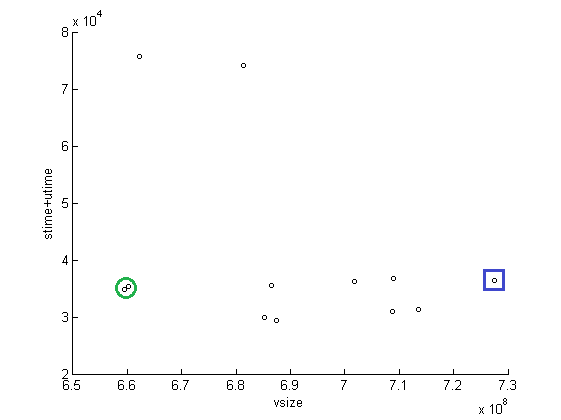
\includegraphics[width=0.8\textwidth]{Ivan_Valencik_RootCnv_opt_vsizeXcpu.png}
  \caption{\small{A relation between memory usage and processor time. The point in the blue square represents the current settings and the points in the green circle represent the ideal settings.}}
\end{center}
\end{figure}

We can also see that switching to the new settings has a positive impact on the memory needed for reading and no obvious or dramatical change of the read time. It is very clear that for reading the basket size has the biggest effect on the memory needed. Big basket sizes are unnecessary.

A significant reduction in memory usage with no drawbacks in processor time or file size in copying and reading suggests that the parameters should be changed. In table \ref{tab:smallvalues} we explore parameter space with low values of basket and tree branch buffer sizes. We can see there that splitting in combination with low basket size has a catastrophic effect on the runtime. Although a configuration with basket size of 1 MB requires even less memory than the one with 2 MB, the best compromise in respect to runtime seems to be a basket size around 2 MB. This value is best combined with a tree branch buffer size of 1 kB.

\section{Conclusion}
\label{sec:conclusion}
In this paper we explained optimization possibilities in ROOT conversion service and introduced a new service for monitoring performance in applications using this service. We also observed real stripping jobs and introduced a test environment that enables to do sweeps over the parameter space. The jobs executed in these sweeps were simulating stripping and further analysis by copying and reading back event data in ROOT files. The performed analysis of the memory footprint indicates a possible gain of 40 MB per output stream without negative effects. This analysis has been done as a part of a Summer Student Programme assignment.

\bibliographystyle{plain}
\bibliography{Ivan_Valencik_RootCnv_opt}

\end{document}
